\documentclass[a4paper]{article}
\usepackage{array}  
\usepackage[table]{xcolor}% http://ctan.org/pkg/xcolor
\usepackage{geometry}
\geometry{margin=1.25in}
\usepackage{hhline}
\usepackage{environ}
\usepackage{graphicx}
\usepackage{float}
 %\geometry{
 %a4paper,z
 %total={170mm,257mm},
 %left=40mm,
 %right=40mm
 %}
 \newcommand{\colWidth}{141mm}

\begin{document} 
\section*{Demo day: \textit{(demo 4)} Group \textit{(group 10)}}

% ------------GOALS----------

\begin{center}
\begin{tabular}{|p{\colWidth}|}
	\hline
	\cellcolor{blue!25}\large
	\textbf{What were your goals?}
	\\ \hline
	\vtop to 100mm{
\begin{itemize}
    \item B.O.B Hardware
    \begin{itemize}
         \item Construct B.O.B shelves.
         \item Improve and finalise B.O.B lift. 
         \item Improve and finalise B.O.B grabber. 
         \item Attach camera to B.O.B.
    \end{itemize}
    \item B.O.B Software
    \begin{itemize} 
        \item Implement B.O.B vision, object detection.
        \item Add bump sensors to stop grabber.
    \end{itemize}
    \item Server: 
    \begin{itemize}
        \item Implement path-finding to allow for multiple items to be picked up.
        \item More integration tests for Server.
    \end{itemize}
    \item App:
    \begin{itemize}
        \item HCI testing and improving App.
    \end{itemize}
    \item Website: 
    \begin{itemize}
        \item HCI testing.
        \item Add descriptive content.
    \end{itemize}
\end{itemize}
  }
  \\
  %have database - connects - get order and stuff - FOR SERVER
  \hline
\end{tabular}
\vskip 5mm

% ------------ORGANISATION----------

\begin{tabular}{|p{\colWidth}|}
	\hline
	\cellcolor{blue!25}\large
	\textbf{Summarise how your group organised the workload to achieve your goals.}
	\\ \hline
	\vtop to 100mm{
	\begin{itemize}
	    \item Team Split
	    \begin{itemize}
	        \item Robot Hardware
	        \item Robot Software
	        \item Server, Website and App 
	    \end{itemize}
	    \item Robot Hardware
	    \begin{itemize}
	        \item Jacob finalised B.O.B's design.
	        \item Jacob and Anna constructed shelves.
	        \item Anna attached camera on B.O.B and soldered cables.
	        \item Kieran decorated B.O.B.
	    \end{itemize}
	    \item Robot Software
	    \begin{itemize}
	        \item Claire and Alex worked on B.O.B's vision.
	        \item Claire added bump sensors for grabbing.
	        \item Freddie assisted with object detection and B.O.B's movement.
	    \end{itemize}
	    \item Server, Website and App 
	    \begin{itemize}
	        \item Oktay did more integration tests for the Server.
	        \item Freddie implemented path-finding for B.O.B to collect multiple items.
	        \item Oktay did HCI testing for the App. Finalised the App after user testing.
	        \item Harry finalised the Website. Added descriptive content to Website and did HCI testing.
	    \end{itemize}
	\end{itemize}
  }
  \\
  \hline
\end{tabular}
\vskip 5mm

% ------------ACHIEVEMENTS----------

\begin{tabular}{|p{\colWidth}|}
	\hline
	\cellcolor{blue!25}\large
	\textbf{What were your main achievements?}
	\\ \hline
	\vtop to 15mm{
	\begin{itemize}
	    \item B.O.B can execute orders and collect multiple items.
	    \item B.O.B can see and detect objects.
	\end{itemize}
  }
  \\
  \hline
\end{tabular}
\vskip 5mm

% ------------NOT ACHIEVED----------

\begin{tabular}{|p{\colWidth}|}
	\hline
	\cellcolor{blue!25}\large
	\textbf{What did you not achieve? Briefly explain why.}
	\\ \hline
	\vtop to 8mm{
	\begin{itemize}
	    \item Environment construction for demo day. Parts for two shelves were not available until just before the demo. (Will be constructed by Thursday.)
	\end{itemize}
  }
  \\
  \hline
\end{tabular}
\vskip 5mm

% ------------NEXT STEPS----------

%\begin{tabular}{|p{\colWidth}|}
%	\hline
%	\cellcolor{blue!25}\large
%	\textbf{Say briefly what changes you will make to your plan for the next demo.}
%	\\ \hline
%	\vtop to 30mm{
%	\begin{itemize}
%	    \item Finalising B.O.B lift system.
%	    \item HCI tests.
%	    \item Unit tests for Website and App. 
%	    \item More integration tests for Server.
%	    \item Adding descriptive content to Website. 
%	\end{itemize}
%  }
%  \\
%  \hline
%\end{tabular}

% ------------QUANTITIVE----------
\newpage
\begin{tabular}{|p{\colWidth}|}
	\hline
	\cellcolor{blue!25}\large
	\textbf{Include any quantitative data you have collected (this can be a graph/table with a few words)}
  \\
  \hline
\end{tabular}

\begin{table}[H]
\centering
\begin{tabular}{| p{2.5cm} | p{1.5cm} | p{1.5cm} | p{2cm} |}
\hline
\textbf{Item} & \textbf{Cost Per Unit} & \textbf{Quantity} & \textbf{Total Cost} \\
\hline
EV3 Colour Sensor & £30.00 & 2 & £60.00 \\
\hline
Omni Wheels & £6.60 & 6 & £39.60 \\
\hline
Hardboards & £14.00 & 2 & £28.00 \\
\hline
Metal Axles & £20.00 & 1 & £20.00 \\
\hline
Website Domain & £1.00 & 1 & £1.00 \\
\hline
Miscellaneous & £10.00 & 1 & £10.00 \\
\hline
Server Cost & £10.00 & 1 & £10.00 \\ 
\hline
 &  & \textbf{Total} & £168.60 \\ 
\hline
 &  & \textbf{Balance} & £31.40 \\
\hline
\end{tabular}
\caption{Finance.}
\end{table}

\begin{figure}[H]
\minipage{0.90\textwidth}
  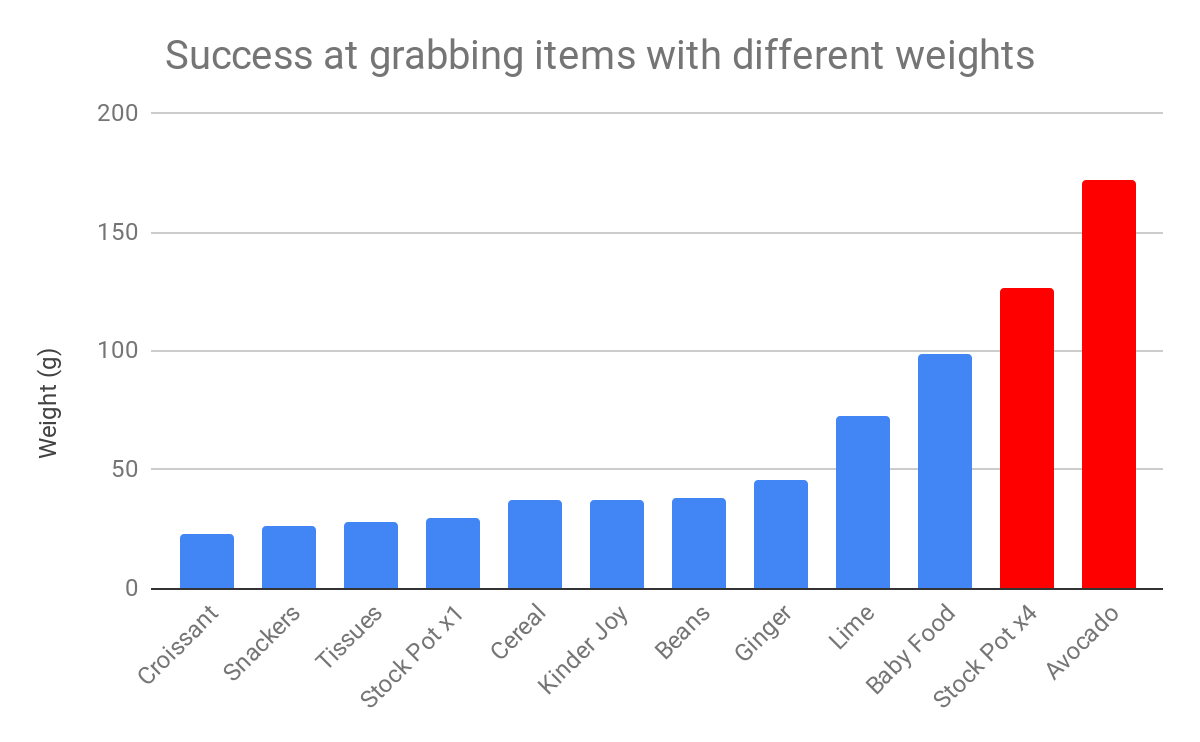
\includegraphics[width=\linewidth]{grab-rate.png}
  \caption{Success rate of grabbing items. Blue = Successful; Red = Failure.}\label{fig:awesome_image1}
\endminipage
\newline
\end{figure}

\begin{table}[H]
\centering
\begin{tabular}{| p{2.5cm} | p{2cm} | p{2cm} | p{2cm} | p{2cm} | p{2cm} |}
\hline
\textbf{Item} & \textbf{Weight (g)} & \textbf{Width (mm)} & \textbf{Depth (mm)} & \textbf{Height (mm)} & \textbf{Rating (S/F)} \\
\hline
Croissant & 23 & 109 & £61 & 41 & Successful \\
\hline
Snackers & 26 & 118 & 112 & 52 & Successful \\
\hline
Tissues & 28 & 55 & 110 & 36 & Successful \\
\hline
Stock Pot (x1) & 30 & 74 & 52 & 35 & Successful \\
\hline
Cereal & 37 & 70 & 104 & 39 & Successful \\
\hline
Kinder Joy & 37 & 70 & 104 & 39 & Successful \\
\hline
Beans & 38 & 81 & 121 & 37 & Successful \\ 
\hline
Ginger & 46 & 94 & 56 & 27 & Successful \\ 
\hline
Lime & 73 & 55 & 45 & 45 & Successful \\
\hline
Baby Food & 99 & 76 & 40 & 134 & Successful \\ 
\hline
Stock Pot (x4) & \textbf{127} & 52 & 146 & 54 & Failure \\
 \hline
Avocado & \textbf{172} & 85 & 58 & 64 & Failure \\ 
\hline
\end{tabular}
\caption{Success rate when grabbing items with different weigths.}
\end{table}

\begin{figure}[H]
\minipage{0.90\textwidth}
  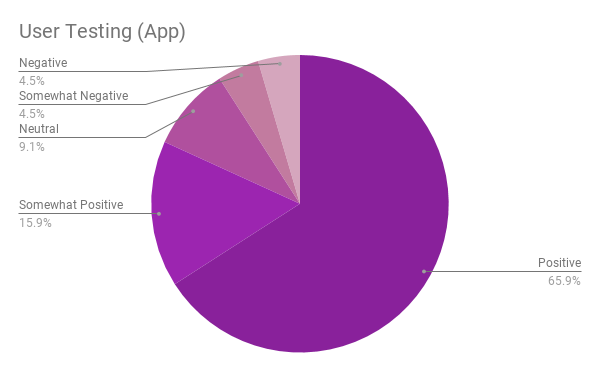
\includegraphics[width=\linewidth]{ease-app.png}
  \caption{Users ratings on App UI.}\label{fig:awesome_image1}
\endminipage
\newline
\end{figure}

\begin{figure}[H]
\minipage{0.90\textwidth}
  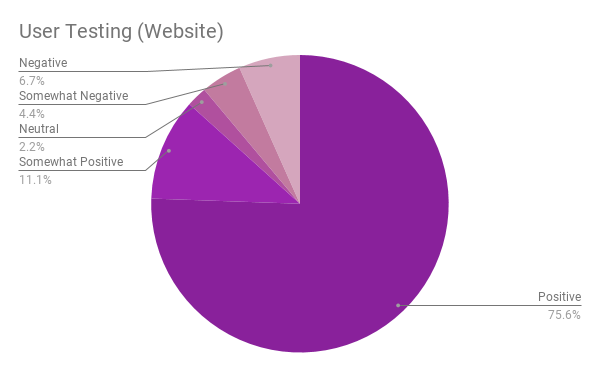
\includegraphics[width=\linewidth]{ease-web.png}
  \caption{Users ratings on Website UI.}\label{fig:awesome_image1}
\endminipage
\newline
\end{figure}

\end{center}
  
\end{document}
